\documentclass[a4paper, 11pt]{article}
\usepackage{comment} % enables the use of multi-line comments (\ifx \fi) 
\usepackage{fullpage} % changes the margin
\usepackage{color,listings,graphicx,float,booktabs,multirow}
\usepackage[colorlinks=true, urlcolor=blue]{hyperref}

\definecolor{codegreen}{rgb}{0,0.6,0}
\definecolor{codegray}{rgb}{0.5,0.5,0.5}
\definecolor{codepurple}{rgb}{0.58,0,0.82}
\definecolor{backcolour}{rgb}{0.95,0.95,0.92}
 
\lstdefinestyle{mystyle}{
    backgroundcolor=\color{backcolour},   
    commentstyle=\color{codegreen},
    keywordstyle=\color{magenta},
    numberstyle=\tiny\color{codegray},
    stringstyle=\color{codepurple},
    basicstyle=\footnotesize,
    breakatwhitespace=false,         
    breaklines=true,                 
    captionpos=b,                    
    keepspaces=true,                 
    numbers=left,                    
    numbersep=5pt,                  
    showspaces=false,                
    showstringspaces=false,
    showtabs=false,                  
    tabsize=2
}
 
\lstset{style=mystyle}

\begin{document}
\graphicspath{{./figures/}}
\noindent
\large\textbf{Kyle Salitrik} \\
\normalsize CMPSC 450\\
\large{Homework 2 Report} \hfill 


\section*{CPU Performance Analysis}
After the corrected code was released, I re-compiled and ran the Vector Triad Benchmark (VTB). The computer used has 16GB of RAM, an Intel i7-6700K processor (4.0 GHz standard clock spee, 4.2 GHz boost speed), and was running Ubuntu 16.04LTS. All compilations were performed with GCC. 

The following table includes information gathered from the Wikipedia article on \href{''https://en.wikipedia.org/wiki/FLOPS''}{\underline{FLOPs}} and \href{''http://ark.intel.com/products/88195/Intel-Core-i7-6700K-Processor-8M-Cache-up-to-4_20-GHz''}{\underline{Intel's}} site.
% Table generated by Excel2LaTeX from sheet 'i7_Specs'
\begin{table}[htbp]
	\centering
	\caption{i7-6700k Specifications}
	\begin{tabular}{lrlr}
		\multicolumn{3}{c}{i7-6700k} &  \\
		Memory Bandwidth          & 34.1 & GB/s       &   \\
		FLOPS                     & 16   & per cycle  &   \\
		Normal CPU Speed          & 4    & GHz normal &   \\
		Boost CPU Speed           & 4.2  & GHz boost  &   \\
		Normal CPU FLOPS          & 64   & GFLOPS     &   \\
		Boost CPU FLOPS           & 67.2 & GFLOPS     &   \\
		Normal CPU FLOPS per Core & 16   & GFLOPS     &   \\
		Boost CPU FLOPS per Core  & 16.8 & GFLOPS     &   \\
		Memory Bandwidth Per Core & 34.1 & GB/s       &   \\
	\end{tabular}%
	\label{tab:addlabel}%
\end{table}%
This figure displays the configuration of the 6th Generation (Skylake) Intel Processors. The L3 cache is 8MB, shared across all four cores. In the above table,the memory bandwidth per core was unavailable, so various calculations were made with assumptions where the memory bandwidth is universal across all cores and if it would be split across cores.
\begin{figure}[H]
	\centering
	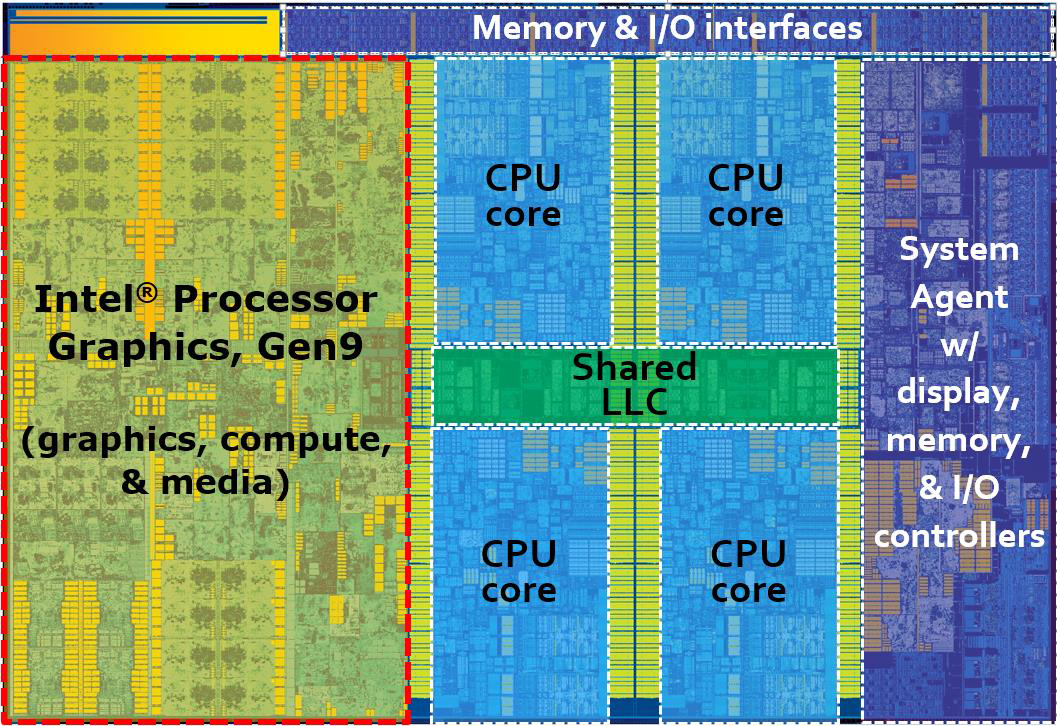
\includegraphics[width=5in]{skylake_diagram.png}
\end{figure}
\newpage
The first table below includes the results for the VTB without any optimization flags passed to the compiler.

\begin{figure}[H]
	\centering
	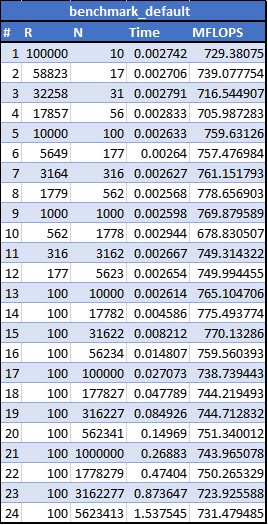
\includegraphics[scale=.75]{vt_base.png}
\end{figure}

The next table shows the results when optimization flags are passed (-O1, -O2, -03) and are marked as such.

\begin{figure}[H]
	\centering
	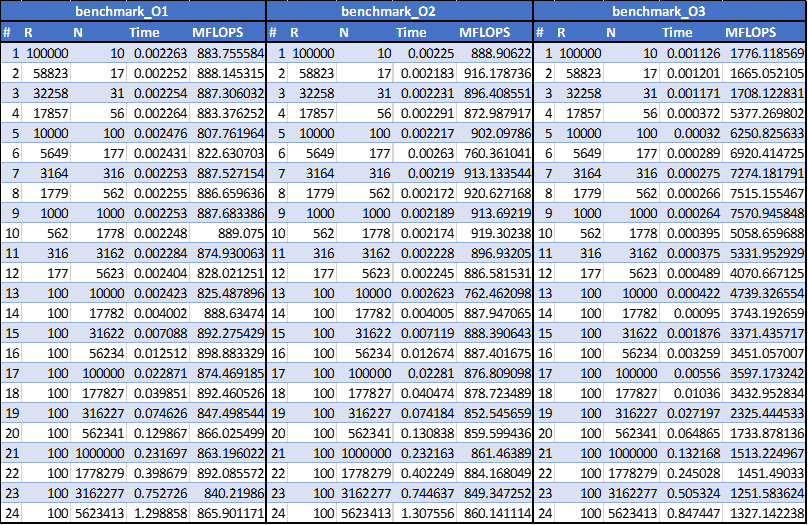
\includegraphics[width=6in]{vt_opt.png}
\end{figure}

The boost to performance with the optimization flags is apparent, however telling the compiler to use SIMD commands (-mavx flag) produces significant increases in throughput as displayed below.
\begin{figure}[H]
	\centering
	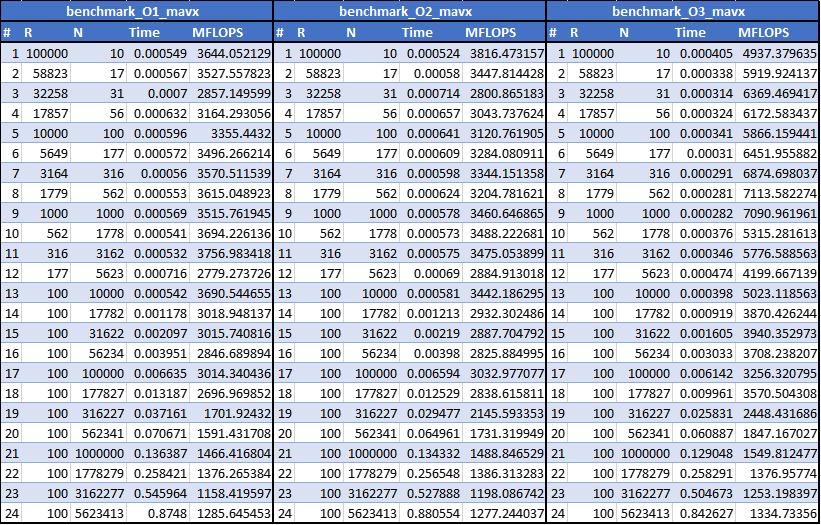
\includegraphics[width=6in]{vt_mavx.png}
\end{figure}

\newpage
This next table shows the estimated performances of the code using the Machine and Code Balance equations provided. The first set of performance results assumed that the full memory bandwidth was available to all cores and the second assumed that the memory balance was split between pairs of cores. The graphs following this table shed more light on the performance of the benchmark.


% Table generated by Excel2LaTeX from sheet 'CPU'
\begin{table}[htbp]
	\centering
	\caption{CPU Performance Calculations}
	\begin{tabular}{lrl}
		Memory Bandwidth        & 4.2625      & Gwords/sec \\
		Peak Performance        & 16          & Gflops/sec \\
		Machine Balance         & 0.26640625  & Words/Flop \\
		                        &             &            \\
		Data Traffic            & 4           & Words      \\
		FLOPS                   & 2           & FLOPS      \\
		Code Balance            & 2           & Words/Flop \\
		                        &             &            \\
		L                       & 0.133203125 &            \\
		p-l*Pmax                & 2.13125     & GFLOPS/Sec \\
		P-bmax/bc               & 2.13125     & GFLOPS/Sec \\
		p-l*Pmax (bandwidth/2)  & 1.06563     & GFLOPS/Sec \\
		P-bmax/bc (bandwidth/2) & 1.06563     & GFLOPS/Sec \\
						    
	\end{tabular}%
	\label{tab:addlabel}%
\end{table}%

This first graph displays the full range of values of N, with the number of MFLOPS stabilizing between 1200-1300, or 1.2-1.3 GFLOPS, which is somewhere in between the estimated performance. Due to this and the advertisement of the Skylake having a "smart allocated cache" it is possible that the cache bandwidth can vary for each core based on the needed throughput. If the assumption that each core received 1/4 of the total bandwidth, the estimate would show the output being close to 500MFLOPS, so that must not be the case.

\begin{figure}[H]
	\centering
	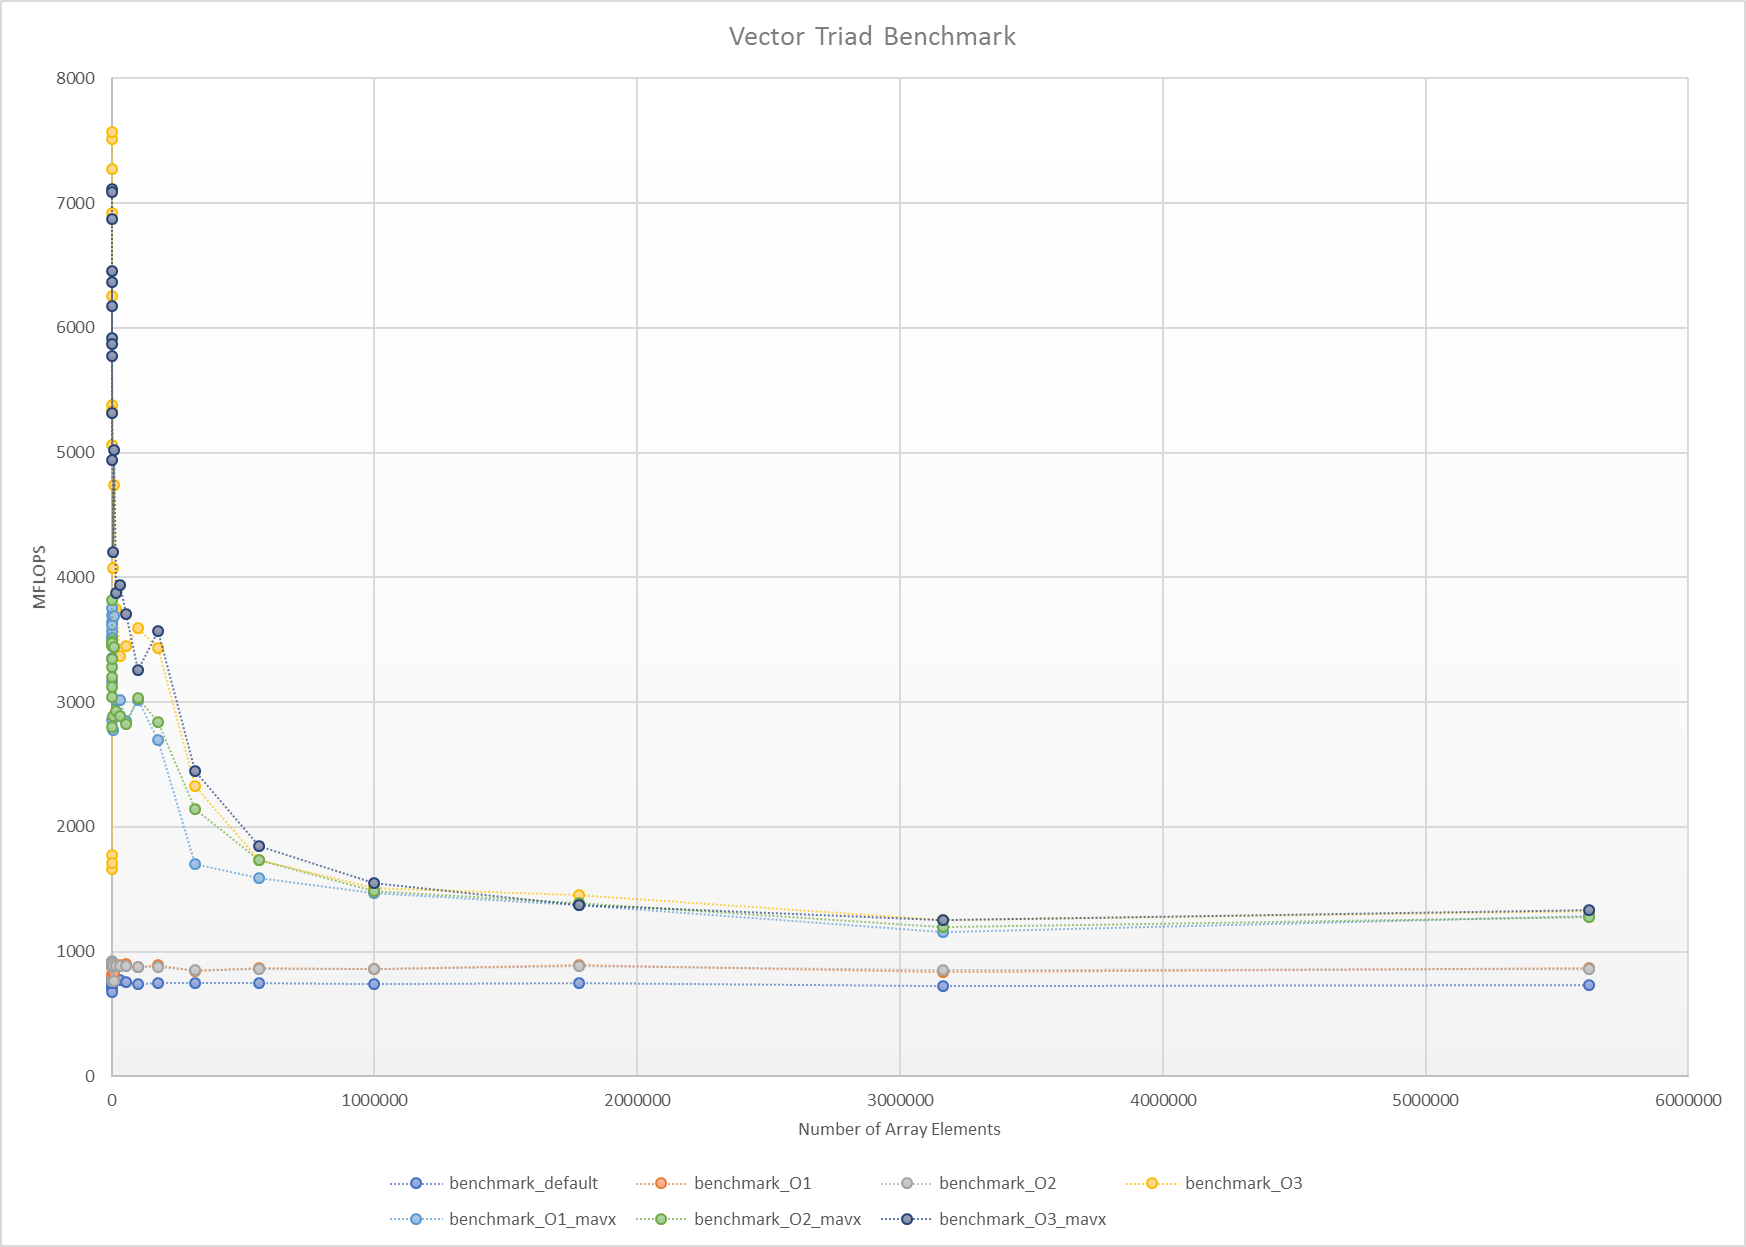
\includegraphics[width=6in]{benchmark_full.png}
\end{figure}

\newpage
This second graph is the same values, trimmed down to N=100k in order to showcase what I assume is where the cpu has run out of cache memory and began to access memory.
\begin{figure}[H]
	\centering
	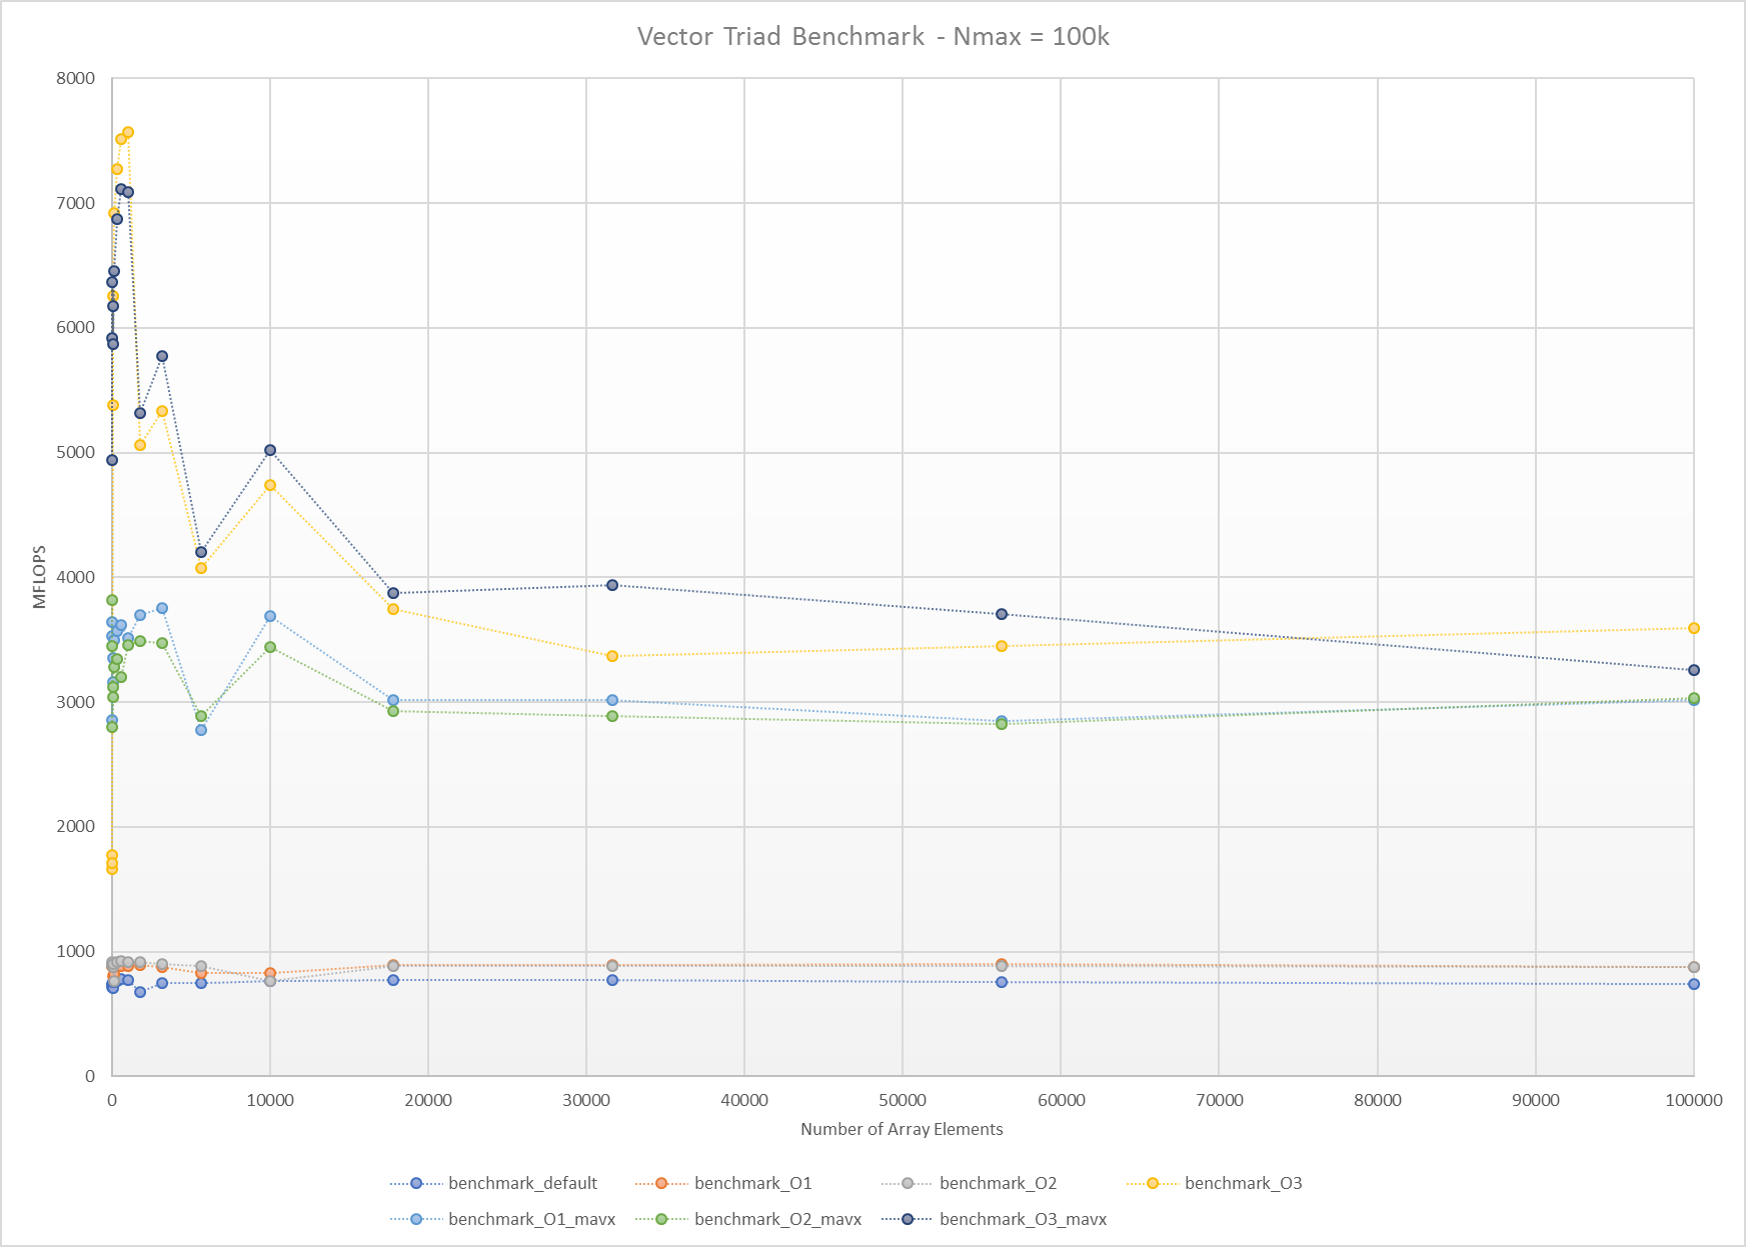
\includegraphics[width=6in]{benchmark_100k.png}
\end{figure}

\newpage

The final graph shows N up to 18,000 in order to observe some of the behavior of the L1, L2 and L3 caches which I assume end around N=1300, N=3000, and N=10,000, respectively, based on the drops in performance that follow the next step. However, to truly rule these out, more finely adjusted values of N would need to be used.
\begin{figure}[H]
	\centering
	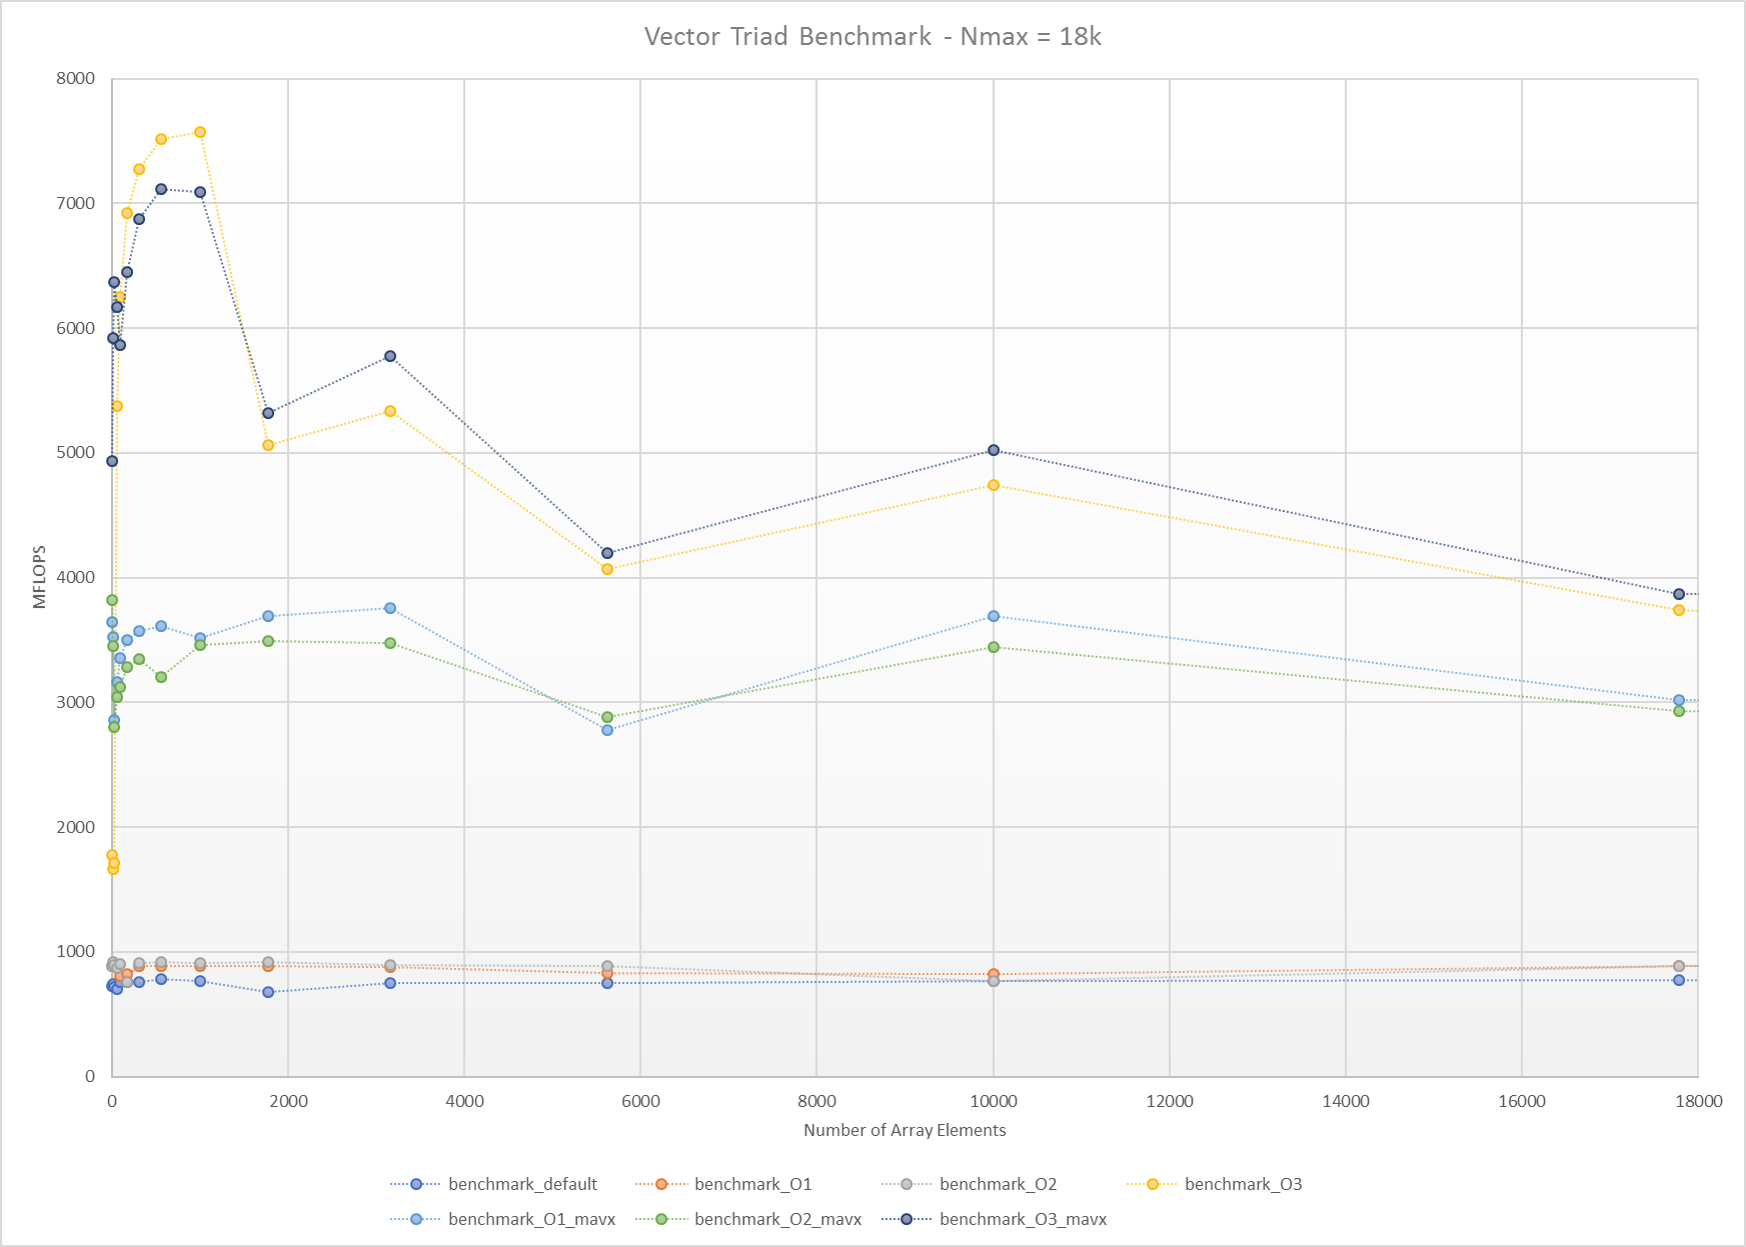
\includegraphics[width=6in]{benchmark_10k.png}
\end{figure}

%====================================================================
\newpage
\section*{Code Optimization}
For the code optimization, I simply moved all of the sine, cosine and floating point operations to a lookup table and populated that before the benchmark loop. I also changed the type of d\_val to integer since there was no point in having an unnecessary floating point operation in the loop. The following table shows the drastic boost in performance gained from simply using this lookup table.
 
% Table generated by Excel2LaTeX from sheet 'Assignment'
\begin{table}[htbp]
	\centering
	\caption{Code Optimization Execution Times}
	\begin{tabular}{lr}
		slow\_default       & 1.074275 \\
		slow\_O1            & 0.661532 \\
		slow\_O2            & 0.652173 \\
		slow\_O3            & 0.651742 \\
		slow\_O1\_mavx      & 0.538004 \\
		slow\_O2\_mavx      & 0.526898 \\
		slow\_O3\_mavx      & 0.544326 \\
		                    &          \\
		optimized\_default  & 0.13495  \\
		optimized\_O1       & 0.018026 \\
		optimized\_O2       & 0.015184 \\
		optimized\_O3       & 0.015131 \\
		optimized\_O1\_mavx & 0.018367 \\
		optimized\_O2\_mavx & 0.011529 \\
		optimized\_O3\_mavx & 0.011716 \\
	\end{tabular}%
	\label{tab:addlabel}%
\end{table}%
 
Finally, the graph below is included in order to visualize the performance increase.
\begin{figure}[H]
	\centering
	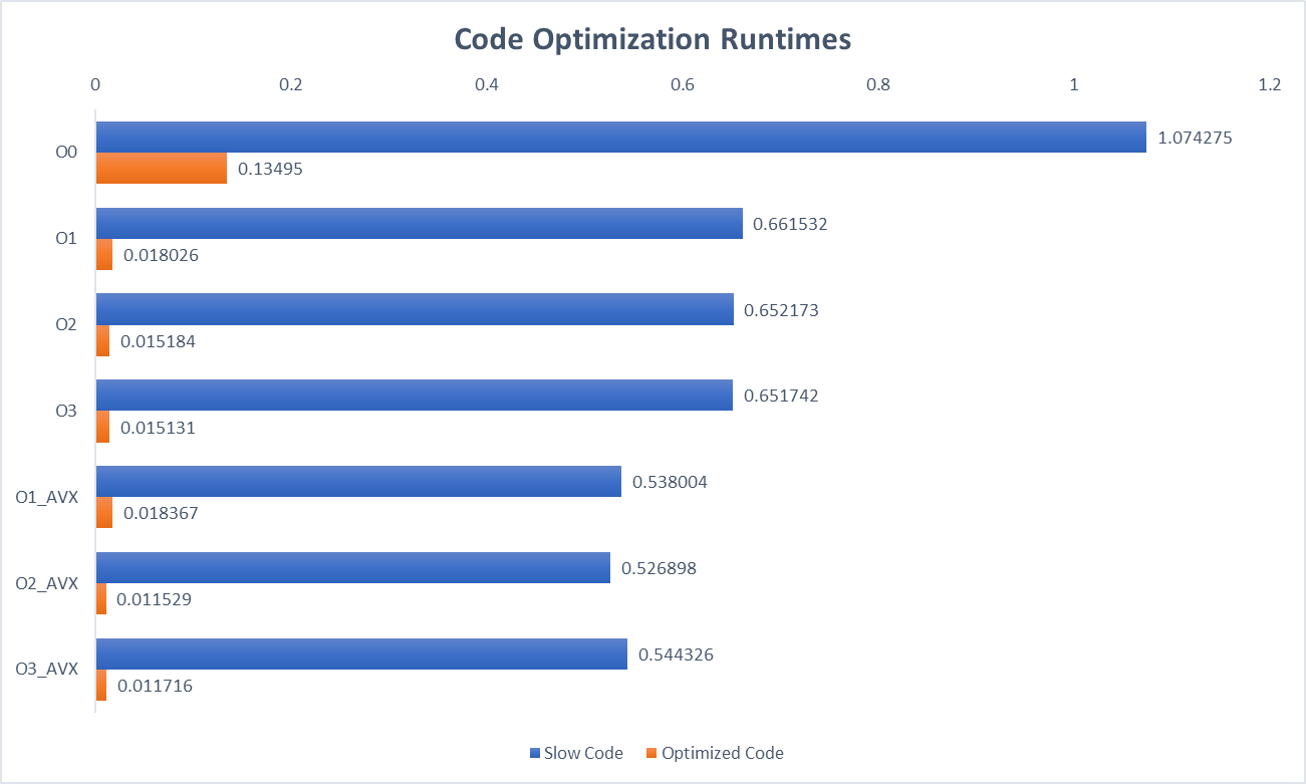
\includegraphics[width=6in]{optimization_runtimes.png}
\end{figure}

%====================================================================
\newpage
\section*{Code Appendix}
\lstinputlisting[language=C++]{../main.cpp}

\end{document}